\icode{E-MI-SI-L3-261106-002}
如图所示，一倾角为\(\theta\)、质量为\(M\)的斜劈始终静止于水平地面上，在其斜面上放有一质量为\(m\)的滑块，其与斜劈之间的动摩擦因数为\(\mu\)，给滑块一沿斜面向下的初速度，滑块减速下滑。已知重力加速度为\(g\)，现对滑块施加一个大小不变的力\(F\)，则在\(F\)由竖直向下逆时针级慢转动到水平向右(如图虚线所示)的过程中，滑块始终在斜面上向下滑，斜劈受到地面的静摩擦力的方向和最大值分别为\paren[]
		
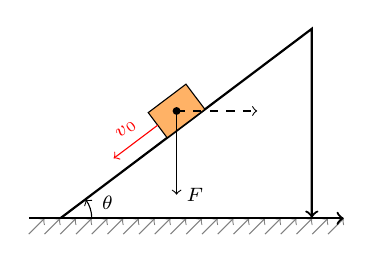
\begin{tikzpicture}[->,font=\scriptsize]
	\begin{scope}[rotate=37]
		\coordinate (O) at(2,.2);
		\draw[thick] (0,0)--(4,0)--++(-127:2.4);
		\draw[fill=orange!60] (1.7,0) rectangle(2.3,.4);
		\draw[->,red] (1.7,.2)--node[above,rotate=37]{\(v_0\)}(1,.2);
	\end{scope}
	\fill (O) circle(.05);
	\draw[->] (O)--(O|-1.5,.3)node[right]{\(F\)};
	\draw[->,dashed] (O)--(O-|2.5,.3);
	\foreach \x in {-.4,-.2,...,3.4}
		\draw[gray] (\x,-.2)--++(.2,.2);
	\draw[thick] (-.4,0)--(3.6,0);
	\draw (.4,0) arc(0:37:.4);
	\node at(.6,.2){\(\theta\)};
\end{tikzpicture}
\begin{choices}
	\item 水平向右，\((mg\cos\theta + F)\cdot(\mu\cos\theta -\sin\theta)\)
	\item 水平向右，\((mg\cos\theta + F\cos\theta)\cdot(\mu\cos\theta -\sin\theta)\)
	\item 水平向左，\((mg\cos\theta + F)\cdot(\mu\cos\theta -\sin\theta)\)
	\item 水平向左，\((mg\cos\theta + F\cos\theta)\cdot(\mu\cos\theta -\sin\theta)\)
\end{choices}
\begin{answer}
	C\qquad 提示：
\end{answer}